% Preheader
%%%%%%%%%%%%%%%%%%%%%%%%%%%%
%%% DOCUMENT
%%%%%%%%%%%%%%%%%%%%%%%%%%%%

\documentclass[12pt,a4paper,captions=tableheading]{article}
% you may add/remove "twoside" above
% or "12pt"



%%%%%%%%%%%%%%%%%%%%%%%%%%%%
%%% TIMES-LIKE FONT
%%%%%%%%%%%%%%%%%%%%%%%%%%%%
\usepackage{mathptmx}



%%%%%%%%%%%%%%%%%%%%%%%%%%%%
%%% FONTS ETC.
%%%%%%%%%%%%%%%%%%%%%%%%%%%%

\usepackage[skip=15pt]{caption}
\usepackage[utf8]{inputenc}
\usepackage[T1]{fontenc}
\usepackage[english]{babel}
\usepackage{amsmath}
\usepackage{amsfonts}
\usepackage{amssymb}

%%%%%%%%%%%%%%%%%%%%%%%%%%%%
%%% CODE HIGHLIGHTING
%%%%%%%%%%%%%%%%%%%%%%%%%%%%
\usepackage{fancyvrb}  
\usepackage{minted} 
\usepackage{helvet}

\usepackage{xcolor}
\definecolor{border}{HTML}{ff5500}

\usepackage{tcolorbox}
\usepackage{etoolbox}
% for angular corners, Argument: arc is angular
\BeforeBeginEnvironment{minted}{\begin{tcolorbox}[colback=white, colframe=border, boxrule=0.4mm, arc=15px]}
\AfterEndEnvironment{minted}{\end{tcolorbox}}

%\setminted{style=abap}
\setminted{style=arduino}
\usepackage{fancyhdr}
%%%%%%%%%%%%%%%%%%%%%%%%%%%
%%% MISC USEPACKAGES
%%%%%%%%%%%%%%%%%%%%%%%%%%%% 
% font to Times
%\fontfamily{ptm}\selectfont
% font Arial

%\renewcommand{\familydefault}{\sfdefault}
% for figures
\counterwithin{figure}{section}
\usepackage{graphicx}
\graphicspath{ {./graphics/} }
% for the Distances
\usepackage[left=1.50cm, right=1.50cm, top=3.00cm, bottom=2.00cm]{geometry}
% für comment section
\usepackage{verbatim}
% für Zeilenabstand 1,5
\usepackage[onehalfspacing]{setspace}
% for spacing \hlines, default was 3pt,
% but led to a weird overall layout
\usepackage{tabularx}
% for long tables
\usepackage{longtable}
% to use the title and author
%\usepackage{titling}
% the options avoid boxes around the links
\usepackage[colorlinks=false, pdfborder={0 0 0}]{hyperref}
% for bibliography
\usepackage[numbers,square,sort]{natbib}
\bibliographystyle{unsrt}
% for subfigures
\usepackage[caption = false]{subfig}
%\usepackage{subcaption}
%for graphic/ table positioning
\usepackage{float}
%Hurenkind und Schusterjunge unterbinden
\usepackage[subfigure]{tocloft}
\clubpenalty=10000
\widowpenalty=10000
%for no shifting at the beginning of paragraph
\parindent 0pt
%for section in equation number
\numberwithin{equation}{section}
% rotating tables
\usepackage{rotating}
% degree
\usepackage{textcomp}
%line overflow handling
\setlength{\emergencystretch}{10em}
% multirow tables
\usepackage{multirow}
% si units
\usepackage[per-mode = fraction, exponent-product = \cdot, locale = DE]{siunitx}
% variable space
\usepackage{xspace}
%for graphic/ table positioning
\usepackage{float}
%für das Einbinden von Tabellen
\usepackage{booktabs}
%quotation
\usepackage{csquotes}
%abkürzungsverzeichnis
\usepackage[printonlyused]{acronym}
\usepackage{booktabs}
\usepackage{enumitem}

\renewcommand{\labelenumii}{\arabic{enumi}.\arabic{enumii}}

%%%%%%%%%%%%%%%%%%%%%%%%%%%%
%%% FORMAT
%%%%%%%%%%%%%%%%%%%%%%%%%%%%

\renewcommand{\cftfigpresnum}{Figure }
\renewcommand{\cfttabpresnum}{Table }
\renewcommand{\listoflistingscaption}{Sourcecode}
\renewcommand{\listingscaption}{Sourcecode}
\renewcommand{\cftfigaftersnum}{:}
\renewcommand{\cfttabaftersnum}{:}

\setlength{\cftfignumwidth}{2.7cm}
\setlength{\cfttabnumwidth}{2.7cm}
\linespread{1.25}
\setlength{\cftfigindent}{0cm}
\setlength{\cfttabindent}{0cm}
% Document

\begin{document}
	
	% Add title without page numbering or any other format
	\pagenumbering{Roman}
	\pagestyle{empty}
	%% Deckblatt
%\thispagestyle{TitelSeite}
\thispagestyle{empty}
\begin{verbatim}


\end{verbatim}

\begin{center}
\large{\textbf{ Development Notes }}

\end{center}

\begin{verbatim}


\end{verbatim}

\begin{center}
	\makebox[\linewidth]{\rule{\linewidth}{0.4pt}}
\end{center}


\begin{center}
	
	\textbf{\LARGE Design and development of an embedded system for controlling RGB LED fixtures}
\end{center}

\begin{center}
	 \large Controlling RGB LED fixtures with dedicated hard- and software subsystems in an combined embedded system
	  \makebox[\linewidth]{\rule{\linewidth}{0.4pt}}
\end{center}

\begin{verbatim}
	
	
\end{verbatim}

\begin{center}
	by Niko Kassubek
\end{center}
%% Ende des Deckblatts

	% Display page numbering
	\pagestyle{plain}

	% Table of contents
	\phantomsection
	\addcontentsline{toc}{section}{Contents}
	\tableofcontents
	\newpage
	
	\renewcommand{\arraystretch}{1.5}
	
	% abbreviations
	%%%%%%%%%%%%%%%%%%%%%%%%%%%%%%%%%%%%%%%%%%
%%%%%%%% INDEX OF ABBREVITATIONS %%%%%%%%%
%%%%%%%%%%%%%%%%%%%%%%%%%%%%%%%%%%%%%%%%%%
\phantomsection
\addcontentsline{toc}{section}{List of Abbreviations}

\section*{List of Abbreviations}
\begin{acronym}[1234567890]\itemsep1pt
	\acro{3D}[3D]{Three-Dimensional}
	\acro{CAD}[CAD]{Computer-Aided Design}
	\acro{DC}[DC]{Direct Current}
	\acro{DCDC}[DC-DC]{Direct Current to Direct Current}
	\acro{DMX}[DMX]{Digital Multiplexing}
	\acro{EEPROM}[EEPROM]{Electrically Erasable Programmable Read-Only Memory}
	\acro{HMI}[HMI]{Human-Machine Interface}
	\acro{HSV}[HSV]{Hue, Saturation, Value}
	\acro{I2C}[I2C]{Inter-Integrated Circuit}
	\acro{IC}[IC]{Integrated Circuit}
	\acro{IO}[I/O]{Input/Output}
	\acro{IP}[IP]{Internet Protocol}
	\acro{LED}[LED]{Light-Emitting Diode}
	\acro{MCU}[MCU]{Microcontroller Unit}
	\acro{OLED}[OLED]{Organic Light-Emitting Diode}
	\acro{PCB}[PCB]{Printed Circuit Board}
	\acro{PWM}[PWM]{Pulse Width Modulation}
	\acro{RGB}[RGB]{Red Green Blue}
	\acro{RS485}[RS485]{Recommended Standard 485}
	\acro{USB}[USB]{Universal Serial Bus}
	\acro{WLAN}[WLAN]{Wireless Local Area Network}
\end{acronym}


	\newpage
	
	\renewcommand{\arraystretch}{1.25}
	% list of figures
	\phantomsection
	\addcontentsline{toc}{section}{\listfigurename}
	\listoffigures
	\newpage

	% list of tables
	\phantomsection
	\addcontentsline{toc}{section}{\listtablename}
	\listoftables
	
	\newpage
	
	% list of Programmcode
	\phantomsection
	\addcontentsline{toc}{section}{Source Code}
%	\lstlistoflistings	
	\listoflistings
	\newpage
	
	% Include the abstract
	%\phantomsection
	%\input{./chapter/abstract}
	%\newpage
	
	% nomenklatur
	%\input{./chapter/nomenklatur}
	%\newpage

	% change page and chaper numbering
	\pagenumbering{arabic}
	\setcounter{section}{0}


	%%%%%%%%%%%%%%%%%%%%%%%%%%%%%%%%%%%%%%%%%%%%%%%
	%%%%%%%%%%  MAIN PART
	%%%%%%%%%%%%%%%%%%%%%%%%%%%%%%%%%%%%%%%%%%%%%%%
	\pagestyle{fancy}
	\fancyhf{} % Clear all header and footer fields
	\fancyhead[C]{\nouppercase{\leftmark}} % Place the current section title on the left side of the header
	\fancyfoot[C]{\thepage} % Place the page number on the right side of the footer
	\renewcommand{\headrulewidth}{0pt} % Optional: Remove the line above the header
	\renewcommand{\footrulewidth}{0pt} % Optional: Remove the line above the footer
	% ADD YOUR CHAPTER HERE
	\section{Introduction}
\label{sec:introduction}
\subsection{Motivation}
\subsection{Problem Statement and Objectives}
\subsection{Structure of the Article}
\textit{(These subsections remain largely the same)}
	\newpage
	\section{Theoretical Background}
\label{sec:theoretical_background}
\subsection{Embedded Systems}
An embedded system is fundamentally a computer system designed for a specific, dedicated function within a larger mechanical or electrical system. It comprises a combination of hardware, typically centered around a processor or \ac{MCU}, memory for storing software and data, and peripheral \ac{IO} devices for interacting with the external environment or the larger system it controls. Unlike general-purpose computers, embedded systems are often constrained by factors such as cost, size, power consumption, and real-time performance requirements, and their software, known as firmware, is specifically tailored to their dedicated task. The \ac{LED} controller developed in this work is an example of such an embedded system.

\subsection{RGB LEDs and Control Methods}
\ac{RGB} \ac{LED}s are semiconductor light sources that combine three individual \ac{LED} elements: red, green, and blue within a single package. By varying the intensity of each primary color, a wide spectrum of colors, including white, can be produced through additive color mixing. Controlling these \ac{LED}s typically involves one of two primary methods relevant to this project. The first method uses \ac{PWM} signals applied independently to each color channel of non-addressable \ac{LED}s, allowing for intensity control of the entire strip or fixture as a single unit. The second method employs addressable \ac{LED}s, where each \ac{LED} (or a small group) incorporates an \ac{IC}. These \ac{IC}s allow the \ac{LED}s to be connected in series and controlled individually via a serial data protocol, enabling complex effects and patterns across the length of an \ac{LED} strip or within a fixture. The choice of control method depends on the specific application requirements, balancing factors like cost, complexity, and the desired level of control granularity.

\subsection{Communication Protocols}
The embedded \ac{LED} controller supports industry-standard communication protocols for receiving lighting control data, enabling integration into various professional and hobbyist setups. Wired communication is primarily handled via the \ac{DMX} protocol, technically known as DMX512. \ac{DMX} is a unidirectional, serial digital protocol transmitted over an \ac{RS485} physical layer, designed for controlling stage lighting and effects. It allows for the addressing and control of up to 512 individual channels within a single "universe," typically corresponding to parameters like intensity or color values for different fixtures. The controller implements \ac{DMX} reception capabilities, allowing it to act as a DMX-controllable device.\\

For network-based control, particularly over wireless networks, the controller utilizes the Art-Net protocol. Art-Net is designed to transmit \ac{DMX} data packets over \ac{IP} networks, leveraging standard networking infrastructure like Ethernet or \ac{WLAN}. This allows for significantly larger systems spanning multiple \ac{DMX} universes and facilitates control from software or consoles connected to the same network. The controller's integrated \ac{WLAN} interface enables it to receive Art-Net commands wirelessly, translating them into the appropriate \ac{LED} output signals. The support for both \ac{DMX} and Art-Net provides flexibility in how the controller is integrated and controlled within a lighting system.

\subsection{User Interface Components}
The primary components facilitating user interaction with the embedded \ac{LED} controller constitute the device's \ac{HMI}. These components allow the user to configure settings, select operating modes, and view status information directly on the device.\\

The main input mechanism is a rotary encoder combined with an integrated push button. This single component serves multiple roles: rotation is used for navigating through menu options or adjusting parameter values, a short press typically confirms a selection or cycles through options within a submenu, and a long press is used to switch between the main menu and submenu levels. This provides a compact and intuitive method for controlling the device's functions without requiring numerous buttons. \\

Visual feedback is provided by a monochrome \ac{OLED} display. This display renders the menu structure, shows current parameter values (such as \ac{HSV} or \ac{RGB} levels, \ac{DMX} addresses, or Art-Net settings), and indicates system status, potentially including connectivity icons or confirmation messages like "Saved". The combination of the rotary encoder input and the \ac{OLED} display output forms the complete local user interface for the controller.

\subsection{Power Supply}
The embedded controller is designed to operate from a flexible main power source, accepting a \ac{DC} input voltage ranging from 12 to 24 Volts via a dedicated connector. Internally, an integrated \ac{DCDC} voltage converter steps this input down to a regulated 5 Volts. This stable 5 Volt supply rail powers the core processing components, including the \ac{MCU} and the \ac{OLED} display. Additionally, the \ac{USB} Type C interface, primarily intended for programming and debugging, can also supply power to the board, typically at 5 Volts, although the main operational power is expected from the 12-24 Volt input.

\subsection{Additive Manufacturing (3D Printing)}\label{subsec:theoretical_3d_printing}
Additive manufacturing, commonly known as \ac{3D} printing, encompasses a set of processes used to create \ac{3D} objects by adding material layer by layer. This approach contrasts fundamentally with traditional subtractive manufacturing methods, which involve removing material from a larger block (e.g., milling or turning). \ac{3D} printing typically starts with a digital model, often created using \ac{CAD} software, which is then sliced into thin cross-sections. The printer deposits, fuses, or solidifies material (such as plastics, resins, metals, or composites) according to these cross-sections, gradually building up the final object. This technology is particularly advantageous for rapid prototyping, creating complex geometries, producing customized parts, and enabling low-volume production runs, such as potentially fabricating custom enclosures or mounting hardware for embedded systems like the one described in this work.

\subsection{Aluminum Extrusion Profiles}\label{subsec:theoretical_aluminum_profiles}
Aluminum extrusion profiles are commonly utilized in mechanical design and construction due to their advantageous properties, including a high strength-to-weight ratio, corrosion resistance, and excellent thermal conductivity. The extrusion process allows for the creation of complex cross-sectional shapes with integrated features like channels, slots, and mounting points. These features make aluminum profiles highly suitable for creating modular and customizable enclosures and structures. In the context of lighting applications, particularly for linear fixtures like the tube light variants developed in this project, these profiles serve multiple purposes. They provide a robust yet lightweight housing, act as an effective heat sink for dissipating thermal energy generated by the \ac{LED}s and electronics, and often include channels designed to hold the \ac{LED} strips, diffusers, and associated \ac{PCB}s securely in place, contributing to a clean and integrated final design.
	\newpage
	\section{System Architecture}
\label{sec:system_architecture}
\subsection{Hardware Core System Block Diagram}
\begin{figure}[H]
	\centering
	\includegraphics[width=0.95\linewidth]{graphics/hardware_architecture}
	\caption{Hardware System Architecture}
	\label{fig:hardwarearchitecture}
\end{figure}
The hardware architecture of the developed embedded \ac{LED} controller is segmented into three primary functional blocks: input, processing, and output. This design facilitates modularity and clear separation of concerns within the system. The schematic representation of this architecture can be seen in the provided diagram.

\subsubsection*{Input Block}

The input block is responsible for receiving power, data, and user commands.

\begin{itemize}
	\item \textbf{Power Supply:} The system accepts a flexible \ac{DC} input voltage ranging from 12V to 24V via a dedicated connector. This allows for compatibility with common power supplies found in lighting applications.
	\item \textbf{Programming and Debugging:} A \ac{USB} Type C interface is incorporated for firmware flashing, debugging, and potential serial communication during development.
	\item \textbf{Wired Communication:} An \ac{RS485} interface enables robust, long-distance wired communication, commonly used for protocols like \ac{DMX} in lighting control. A notable feature is an integrated switch to engage or disengage a 120 Ohm termination resistor, crucial for maintaining signal integrity in \ac{RS485} networks.
	\item \textbf{User Interface:} Direct user interaction is managed by a rotary encoder equipped with a push-button function. This allows users to navigate menus displayed on the \ac{HMI} and confirm selections.
	\item \textbf{Wireless Communication:} The controller integrates a 2.4 GHz \ac{WLAN} interface, enabling it to connect to standard wireless networks. This facilitates wireless control primarily through the Artnet protocol, a common standard for transmitting \ac{DMX} data over Ethernet networks.
\end{itemize}

\subsubsection*{Processing Block}

The processing block handles power regulation and executes the core logic of the controller.

\begin{itemize}
	\item \textbf{Power Conversion:} An essential component is the 5V DC-DC converter. This module steps down the incoming 12/24V supply to a regulated 5V. This stable 5V rail powers the sensitive electronic components, including the microcontroller and the display. \\
	For the spotlight a DC-DC converter provides a 12 V power rail. In this case, the input voltage does not match the fan voltage and is therefore needed. 
	\item \textbf{\ac{MCU}:} The central processing unit is the Seeedstudio XIAO ESP32-C3 microcontroller. This \ac{MCU} was chosen for its integrated Wi-Fi capabilities, sufficient processing power for handling communication protocols and control algorithms, and its compact form factor. It executes the firmware that manages inputs, processes control data (e.g., Artnet, \ac{DMX}), and drives the outputs.
\end{itemize}

\subsubsection*{Output Block}

The output block interfaces with the external components that the controller manages.

\begin{itemize}
	\item \textbf{\ac{LED} Control:} The primary function is controlling \ac{LED} hardware. The system is designed to support two main methods: direct serial communication for addressable \ac{LED} strips and \ac{PWM} control for driving different color channels (e.g., \ac{RGB}) of non-addressable \ac{LED}s.
	\item \textbf{Display Interface:} An \ac{I2C} interface is utilized to communicate with the \ac{OLED} display, which serves as the \ac{HMI}. In certain product configurations, such as integrated panel lights, this \ac{I2C} bus may also be used to send control data to other integrated components. An \ac{I2C} level converter is included to shift voltage levels between the 3.3V logic of the \ac{MCU} and the 5V requirement of the other peripherals. The display works with either 3.3V logic or 5V. To only drive the display, the level converter is not needed.
	\item \textbf{Thermal Management:} To ensure reliable operation, the controller incorporates fan control via a standard \ac{PWM} interface, compatible with typical computer fans. This allows the system to regulate its temperature under load.
\end{itemize}

\subsection{Hardware Configuration Options}
While the core architecture remains consistent, different hardware configurations and \ac{PCB}s are available to suit various application requirements:

\begin{itemize}
	\item \textbf{Tube Light V2 (Non-Addressable \ac{LED}s):} This variant utilizes hardware supporting three \ac{PWM} outputs for controlling non-addressable \ac{LED} strips. It omits the fan control output as it's not typically required for this configuration.
	\item \textbf{Tube Light V3 (Addressable \ac{LED}s):} For tube lights using addressable \ac{LED}s, the hardware provides support for a serial data output. Similar to the non-addressable version, fan control is not included.
	\item \textbf{Panel Light:} This configuration uses the same fundamental hardware as the addressable \ac{LED} tube light (serial output capable). However, the \ac{RGB} data for the panel is specifically transmitted via the \ac{I2C} interface instead of the dedicated serial \ac{LED} output. This version includes the hardware connection for fan control.
	\item \textbf{Spot Light:} The spot light employs an individual \ac{PCB} design tailored to its needs. It features three \ac{PWM} outputs for \ac{LED} control and includes the hardware connection for fan control.
	The size of the \ac{PCB} is designed to fit within the casing. The previous \ac{PCB} would not fit.
\end{itemize}

These variations ensure that each product type has an optimized hardware platform based on the core controller design, omitting unnecessary components or adapting interfaces as needed for the specific application.

\subsection{Software Architecture}
\subsubsection{Overview} 
The software architecture utilizes a hybrid execution approach to balance responsiveness with high-throughput data processing. Asynchronous user inputs and low-frequency tasks, such as display updates or button presses, are handled via an event management system. Conversely, high-frequency tasks requiring immediate execution are managed through continuous polling. Additionally, a software timer module is integrated to inject time-based triggers into the event queue.

\subsubsection{Event Management} 
The system implements an event manager utilizing a \ac{FIFO} buffer to store and sequence system events. These events are retrieved and processed sequentially within the main loop via the \textit{process\_event} function. Event definitions and properties are isolated in specific configuration files, facilitating modular adjustments.
Within sourcecode section \ref{pc:event_manager_config} such a configuration can be seen. 

\begin{listing}[H]
	\begin{minted}[autogobble, linenos=true, numberblanklines=true, frame=leftline, framesep=5pt, numbersep=5pt, style=vs, tabsize=2, xleftmargin=10pt, breaklines, fontsize=\small, baselinestretch=1.0, escapeinside=!!]{c}
		const event_cfg_t event_config[] = { 
			// ID Name Priority Queueable {EVT_NONE, "None", EVT_PRIORITY_LOW, false},
			// Input events
			{EVT_ENCODER_CHANGED, "EncoderChanged", EVT_PRIORITY_HIGH, true},
			{EVT_BUTTON_CLICK, "ButtonClick", EVT_PRIORITY_HIGH, false},
			// System events
			{EVT_SAVE_TO_NVM, "SaveToNvm", EVT_PRIORITY_NORMAL, false},
			{EVT_DISPLAY_WAKE, "WakeUpDisplay", EVT_PRIORITY_NORMAL, false},
		};
	\end{minted}
	\caption{Configuration of the event manager system}
	\label{pc:event_manager_config}
\end{listing}

It is possible for the handling of one event to trigger the posting of subsequent events. This capability must be utilized cautiously to prevent the creation of infinite feedback loops where events recursively trigger one another.

\subsubsection{Software Timer Management} 
Software timers are employed to generate events based on time intervals, operating with a time base of 1 ms. The TimerManager checks all active timers for expiry during every iteration of the main loop. Upon expiry, the manager automatically adds the associated event to the FIFO queue. The system supports two operational modes: 

\begin{itemize} 
	\item \textbf{Periodic:} The timer automatically reloads and restarts after expiry. 
	\item \textbf{One Shot:} The timer is disabled immediately after the expiry event is generated.
\end{itemize}
Similar to the configuration of the event manager, the software timers can be configured through a list. 
Each entry represents one timer configuration. 

\subsubsection{Menu Structure}
User interaction with the device primarily occurs through the rotary encoder and its integrated push button, as depicted in the menu structure diagram figure \ref{fig:menustructure}.
\begin{figure}[H]
	\centering
	\includegraphics[width=0.95\linewidth]{graphics/menu_structure}
	\caption{Structure of the main menu navigation}
	\label{fig:menustructure}
\end{figure}

In the main menu view, turning the rotary encoder allows the user to cycle horizontally through the available function selections (such as \acs{HSV}, \ac{RGB}, \ac{DMX}, Artnet, and Options). The selection does not jump from the last to the first or from the first to the last entry of the menu. 
At both ends an end mark is displayed as user information. \\

Vertical navigation between the main menu level and the corresponding submenu pages is achieved via a long press on the encoder's button. Performing a long press while a main menu item is selected transitions the software into that item's specific submenu, displaying its parameters or options. Conversely, performing another long press while within a submenu returns the user to the main menu selection screen. This hierarchical navigation, visually represented in the provided diagram, allows access to different functionalities and their settings using simple rotary and press actions.
	\newpage
	\section{Hardware Development}
\label{sec:hardware_development}

\subsection{Common Hardware Packages and Components}

The controller board integrates several key hardware packages to realize its functionality. For the \ac{DMX} interface, standard \ac{RJ45} connectors are utilized for physical connectivity. The electrical interface is managed by an SN75176 differential bus transceiver \ac{IC}, which is a common choice for \ac{RS485} communication. To ensure compatibility between the 5V levels of the transceiver and the 3.3V logic level of the \ac{MCU}, a voltage divider circuit is implemented for the data lines. \\

Power regulation is achieved using a switching buck converter, a type of \ac{DCDC} converter, to efficiently step down the input voltage to a stable 5V for the system components. The central processing unit selected for this design is the Seeedstudio XIAO ESP32-C3 \ac{MCU}, which provides the necessary computational power, memory, and peripheral interfaces, including \ac{WLAN} connectivity. User input is primarily handled by a rotary encoder, allowing for menu navigation and parameter adjustment. Visual feedback for the \ac{HMI} is provided by an \ac{OLED} display with a resolution of 128x32 pixels, which communicates with the \ac{MCU} via the \ac{I2C} protocol.

\subsection{Hardware Variations for Light Tube}
The project includes different hardware iterations for the tube light fixtures, primarily differing in their \ac{LED} control methodology:

\begin{description}[style=nextline]
	\item[Light Tube V2] This version employs \ac{MOSFET}s to drive the \ac{RGB} \ac{LED}s of the entire tube. Control is achieved using \ac{PWM} signals for each color channel (Red, Green, and Blue), allowing the overall color and intensity of the tube to be adjusted as a single unit.
	\item[Light Tube V3] This iteration advances to addressable \ac{LED} segments. It utilizes a serial communication protocol, similar to that used by the WS2811 \ac{IC}, to set the color of individual \ac{LED} segments within the tube. This enables more complex lighting effects and patterns by controlling different parts of the tube independently.
\end{description}

\subsection{Hardware Variation for Panel}
The Light Panel variant incorporates several distinct design features tailored to its specific application and components. Thermal management for the densely packed \ac{LED}s and associated electronics is addressed by an 80mm cooling fan mounted on the rear of the panel. This fan's speed is regulated via a \ac{PWM} signal from the main controller, allowing for dynamic adjustment of airflow based on thermal load, thereby optimizing cooling performance while minimizing acoustic noise. \\

For distributing lighting information, the panel employs a hierarchical control system. The \ac{MCU} communicates lighting commands to five independent section control units using the \ac{I2C} protocol. These section control units are built around an ATtiny402 \ac{MCU}. Each of these dedicated section controllers is then responsible for driving a bank of 75 WS2815 \ac{RGB} \ac{LED} \ac{IC}s. Within each section, all 75 \ac{LED}s display the same color, as dictated by their respective section controller, allowing for five distinct color zones across the panel. \\

A notable characteristic of this panel variant is its power system. It operates on a 12 Volt input voltage, distinguishing it from other devices in the project that use 24 Volts. This 12V supply is particularly suitable as the WS2815 \ac{LED} \ac{IC}s are designed to be directly powered from a 12V source. This simplifies the power distribution to the \ac{LED}s, potentially reducing the need for additional voltage regulation steps for the \ac{LED} drivers themselves, although the section control units and main \ac{MCU} would still require appropriate voltage levels (e.g., 3.3V or 5V) derived from this main 12V input.

\subsection{Hardware Variation for Spotlight}
This spotlight device incorporates several key design elements. Effective thermal management is achieved through the use of a dedicated aluminum heatsink, which is actively cooled by an attached fan; this is crucial for dissipating the heat generated by the high-power light source. For the 12V fan a separate power rail is used. The fan is controlled via a \ac{PWM} signal depending on the intensity of the light output.\\

The electronics are housed on a custom \ac{PCB}, specifically designed to conform to the physical dimensions and layout requirements of the fixture. The primary light source is a multi-color \ac{RGB} \ac{COB} \ac{LED} chip, which provides a dense array of \ac{LED}s for bright and uniform color output. Each color channel (Red, Green, and Blue) of this \ac{COB} chip is individually controlled via \ac{PWM} signals, allowing for precise color mixing and intensity adjustment. To shape and direct the light output, the fixture is equipped with a lens designed to focus the beam to a 60° angle, providing a defined area of illumination.

\subsection{Schematic Design}
The initial phase of the \ac{PCB} design involves the detailed creation of schematics using specialized \ac{EDA} software. For this project, schematics have been developed using Autodesk Fusion 360, which integrated the capabilities of the formerly separate Autodesk Eagle software, alongside KiCad version 8. A long-term decision has been made to transition future design work predominantly to KiCad 8, leveraging its open-source nature and comprehensive feature set. \\

Within these software environments, the process includes the careful selection and placement of correct component footprints, which accurately represent the physical dimensions and pin configurations of the parts to be used. If standard footprints are unavailable or unsuitable, custom ones are created. Following this, all necessary logical electrical connections between the components are meticulously drawn, defining the complete circuit topology and its intended behavior. \\

A crucial aspect of the design workflow is the reliance on prior experimental validation. The schematics are not merely theoretical constructs but are developed based on the outcomes of thorough testing and experimentation conducted on breadboard prototypes. This practical approach ensures that the fundamental functions of the circuit and the interplay of its components are proven to be working correctly in a tangible, albeit less permanent, setup. By verifying the design's efficacy at the breadboard stage, the risk of errors in the final \ac{PCB} is significantly mitigated, thereby increasing the confidence in ordering and fabricating \ac{PCB}s that will function as intended from the outset.

\subsection{PCB Design and Fabrication}
The design and fabrication of the \ac{PCB}s for this project adhere to several critical considerations to ensure functionality, reliability, and seamless integration within the overall mechanical design. The physical dimensions of each \ac{PCB} are meticulously planned to fit within the specific mechanical parameters and size constraints dictated by the intended enclosure or mounting arrangement. \\

Careful attention is given to the layout of conductive pathways, with adequate track widths employed for both power and signal lines. Power traces are dimensioned to handle the expected current loads without significant voltage drop or excessive heat generation, while signal traces are routed to maintain signal integrity and minimize noise coupling. \\

Components are strategically placed on the board in logical groups, taking into account their functional relationships as well as the placement of input and output connectors to facilitate straightforward wiring and interaction. Furthermore, informative labels and markings are included on the \ac{PCB} silkscreen layer to display crucial information, such as component designators, polarity indicators, or operational notes like the on/off position for a termination resistor switch. To ensure robust mechanical assembly, mounting holes are strategically placed to align with the mechanical design of the enclosure or support structure. \\

All custom \ac{PCB}s utilized throughout this project are fabricated by the external manufacturing service, JLCPCB. This approach allows for access to professional-grade \ac{PCB} production. A specific consideration applies to the \ac{LED} panel variant: due to the high density of surface-mount \ac{LED}s, the WS2815 \ac{LED} components for these panels are assembled onto the \ac{PCB}s directly by JLCPCB as part of their component assembly service. This outsourcing of the \ac{LED} placement significantly saves time for the assembly process for this particular component-dense design. Further details regarding the overall component assembly process for all boards are provided in a subsequent chapter \textit{\ref{sec:component_assembly} \nameref{sec:component_assembly}}.

\subsection{Component Selection and Justification}

\subsection{Component Assembly}\label{sec:component_assembly}
The assembly of the \ac{PCB}s involves distinct stages for \ac{SMD} and \ac{THT} components, employing manual and semi-automated techniques to ensure reliable solder joints and functional boards. \\

\begin{description}[style=nextline]
	\item[\ac{SMD}] The \ac{SMD} assembly process commences with the application of solder paste to the pads on the \ac{PCB}. A stencil, precisely aligned with the \ac{PCB} footprint, is used to ensure accurate deposition of the paste. To achieve consistent solder paste distribution and ensure repeatability across multiple boards, a temporary jig or contraption is constructed. This setup, typically involving securing the stencil with tape and using other \ac{PCB}s as shims, guarantees the correct height and alignment for an even application. Following solder paste application, the individual \ac{SMD} components are meticulously placed onto their designated positions on the \ac{PCB} using a pair of tweezers. Once all components are placed, the entire assembly is subjected to a reflow soldering process using a hot plate. The controlled heating profile of the hot plate melts the solder paste, allowing it to flow and form robust electrical and mechanical connections between the components and the \ac{PCB}. After the board has cooled, a cleaning step is performed using \ac{IPA} and a brush to remove any flux residues or solder debris, ensuring optimal electrical performance and a professional finish.
	
	\item[\ac{THT}] Subsequent to the completion of the \ac{SMD} assembly and reflow process, the \ac{THT} components are manually soldered to the \ac{PCB}. This step is generally performed for all \ac{THT} parts with the notable exception of the \ac{MCU}, which is handled with additional precaution. Before the \ac{MCU} is installed, a critical verification step involves testing the output of the onboard 5V buck \ac{DCDC} converter. The voltage is carefully measured using a multimeter to confirm it is within the correct operational tolerance. Only if this voltage measurement is confirmed to be fine is the \ac{MCU} then soldered onto the board. This sequenced approach, prioritizing the verification of power rails before installing sensitive components like the \ac{MCU}, minimizes the risk of damage due to power supply faults.
\end{description}

	\newpage
	\section{Mechanical Design and Enclosure}
\label{sec:mechanical_design}

\subsection{Manufacturing Technologies and Materials}
\label{subsec:manufacturing_tech}
The mechanical construction of the RLCV3 system relies on a combination of additive manufacturing, standardized metal components, and specialized fastening techniques to achieve a robust and professional assembly.

\subsubsection{Additive Manufacturing (3D Printing)}
The fabrication of custom enclosures, structural brackets, and end caps is performed using \ac{FDM}.
A BambuLab X1C printer, equipped with a textured \ac{PEI} build plate, is utilized to ensure consistent adhesion and a high-quality surface finish.\\ 

Two primary thermoplastic filaments are employed based on the functional requirements of the components:
\begin{itemize}
	\item \textbf{BambuLab PLA-Basic}: This material is used for the majority of the structural parts, including the main PCB enclosures, as well as the housing components for the Spotlight and Panel variants \cite{inet:bambulab_pla}.
	It offers a favorable balance of rigidity and dimensional accuracy.
	\item \textbf{BambuLab PLA-CF}: A Carbon Fiber reinforced \ac{PLA} composite is utilized for the tube light end caps \cite{inet:bambulab_placf}.
	The addition of carbon fiber enhances the stiffness of the parts and provides a distinctive matte surface finish, contributing to the aesthetic quality of the visible components.
\end{itemize}

To ensure mechanical integrity, specific print parameters are strictly adhered to.
Components are fabricated using a 0.4 mm nozzle with a layer height of 0.12 mm, allowing for fine detail resolution.
Structural strength is prioritized through the use of increased wall thickness rather than high infill density.
Parts are typically sliced with 3 to 4 wall perimeters and 2 to 3 top and bottom layers.
The infill density is set between 20\% and 30\%, utilizing 3D-honeycomb or cubic patterns to provide isotropic strength distribution.
Components subjected to higher mechanical stress, such as the connector systems detailed in section \ref{subsec:connection_systems}, are designed with significantly thicker walls to withstand operational loads.

\subsubsection{Fastening Technology}
To ensure durability and serviceability, the assembly avoids the use of direct threading into plastic or loose nuts.
Instead, brass threaded inserts (typically M3) are integrated into the 3D-printed components.
These inserts are installed using a heat-set process, where a soldering iron is used to melt the plastic locally, allowing the knurled insert to sink into the part and bond securely upon cooling.
This method provides medium pull-out resistance and torque capability \cite{inet:cnckitchen_inserts}.
Furthermore, it simplifies the assembly process by eliminating the need for a counter-wrench and allows for repeated disassembly without degrading the fastening interface.

\subsubsection{Aluminum Extrusion Profiles}
The core structure of the light tube variants is formed by an extruded aluminum U-profile \cite{inet:alu_profile_amazon}.
This profile serves a dual purpose: it acts as the rigid chassis for the fixture and functions as a passive heatsink for the LED strips \cite{inet:alu6063_properties}.
The selected profile features a width of approximately 27 mm and a height of 12 mm.
Originally supplied in 2-meter lengths, the profiles are cut to 1 meter.
Light diffusion is achieved via a compatible milky-white diffuser cover, which snaps into the profile and adds 13 mm to the total height.
Although specific manufacturer data regarding the thermal resistance and structural modulus of this profile is unavailable, empirical testing has confirmed its suitability for dissipating the thermal load generated by the LEDs in this application.
The precise dimensions provided by the manufacturer, as well as the profile cross-section, can be seen in figure \ref{fig:aluprofileedgy}.

\begin{figure}[H]
	\centering
	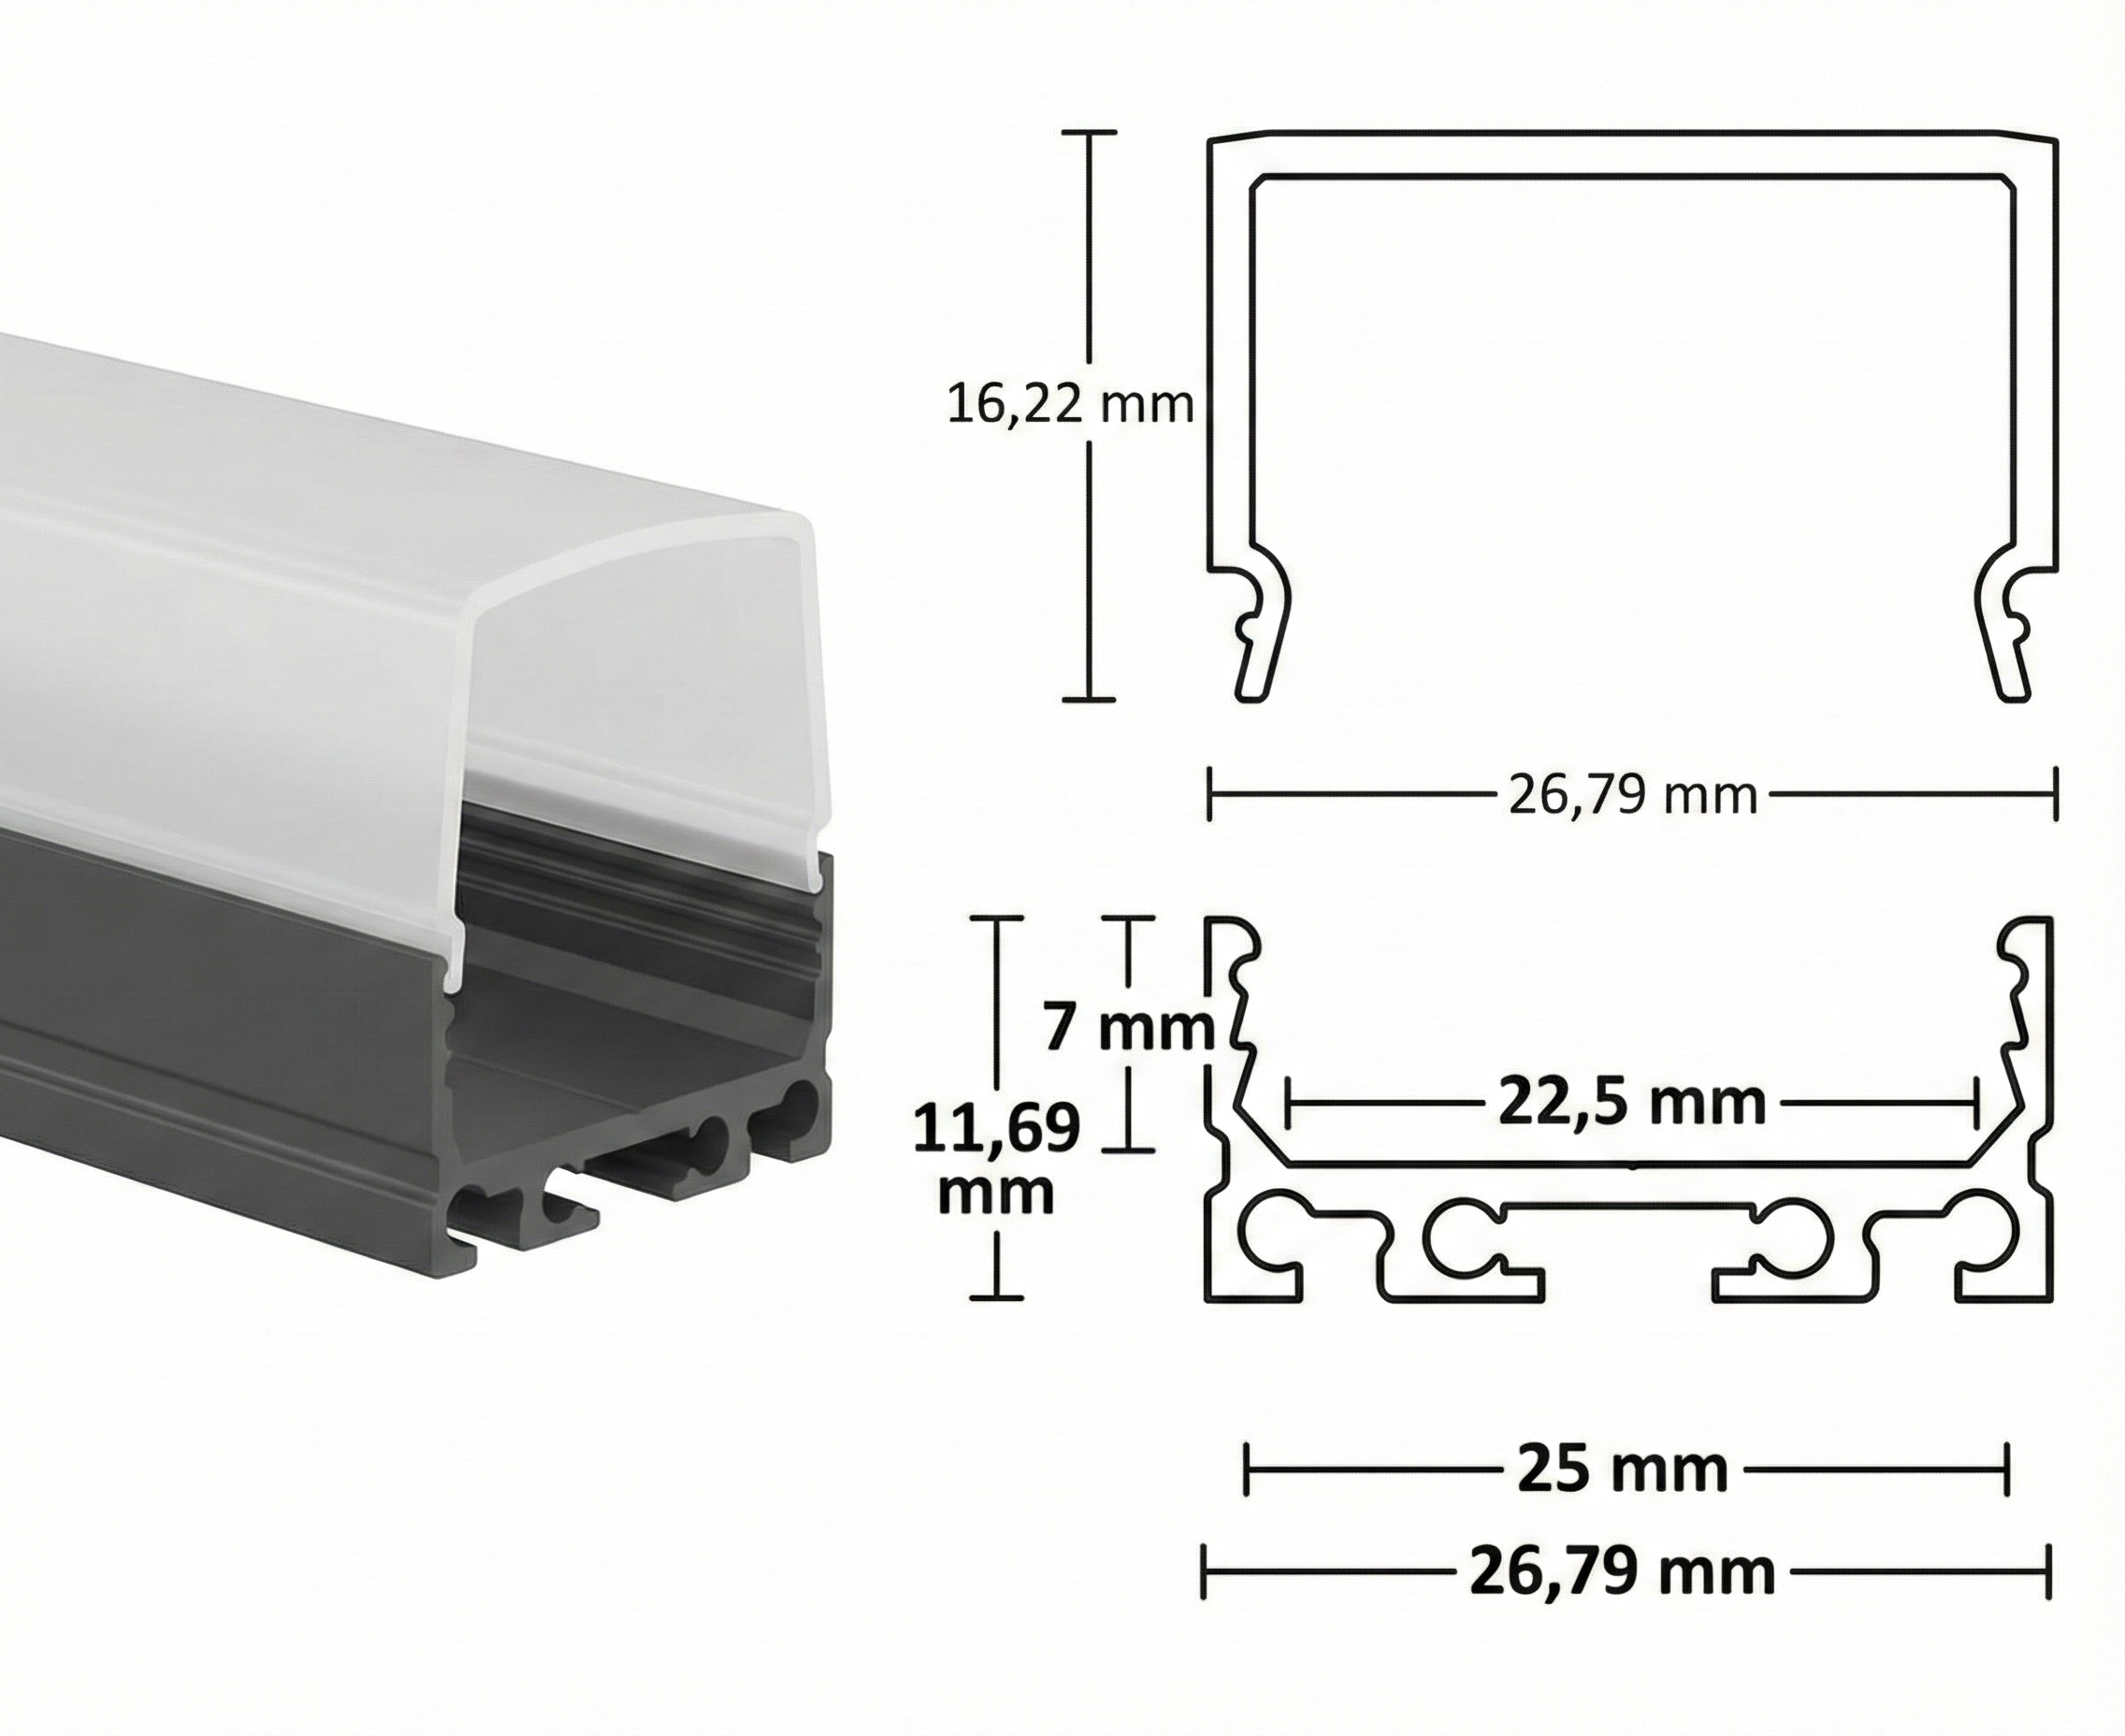
\includegraphics[width=0.6\linewidth]{graphics/alu_profile_edgy}
	\caption{Cross-section of the aluminum U-profile used for the tube light structure.}
	\label{fig:aluprofileedgy}
\end{figure}

\subsection{Light Tube Enclosures}
\label{subsec:light_tube_enclosures}
	Holes are drilled through the aluminum profile, and screws are inserted from the inside channel (the surface to which the \ac{LED} strip is adhered).
	These screws engage with the threaded inserts installed in the 3D-printed parts.
	This approach ensures a clean exterior finish with no visible screw heads on the printed parts and provides a secure mechanical connection.
	Typically, each major component is secured with four screws to prevent rotation and ensure structural rigidity.

\subsubsection{Variant V2 (MOSFET)}
\label{subsubsec:light_tube_v2}
In the V2 iteration, the mechanical design integrated the controller housing directly into one of the end caps.
This single-piece assembly served as both the termination for the tube and the enclosure for the \ac{PCB}.
Mechanical mounting for the fixture was provided via a standard tripod screw thread embedded in the housing.
However, this design lacked the modularity required for more advanced mounting scenarios.
Consequently, this mechanical configuration is considered deprecated.
The V2 electronic hardware is compatible with the improved V3 mechanical design, and therefore, no further development is being conducted on the specific V2 enclosure geometry.

\subsubsection{Variant V3 (Addressable)}
\label{subsubsec:light_tube_v3}
The V3 design represents the current standard for the light tube fixtures, featuring a more modular and robust architecture.
The assembly consists of distinct end caps at both the top and bottom of the tube, which incorporate mechanical interfaces for the connector systems.\\

The controller electronics are housed in a dedicated, two-part enclosure mounted along the length of the profile, rather than at the end.
This enclosure comprises a base plate, which is bolted to the aluminum profile and supports the \ac{PCB}, and a removable lid.
The lid protects the electronics while providing necessary apertures for the \ac{OLED} display, input connectors, and the rotary encoder.\\

Electrical connection between the external controller and the internal \ac{LED} strip is achieved by routing three separate cables through drilled holes into the profile's interior.
To facilitate precise assembly, a 3D-printed drill template is available, allowing the user to accurately mark all 14 required holes: 12 for mechanical fastening of the components and 2 for wire feed-throughs.
Inside the profile, a specialized clip is used to secure the data wire.
This clip is designed to be held in place by the adhesive backing of the \ac{LED} strip itself, ensuring the internal wiring remains unobtrusive and does not cast shadows on the diffuser.\\

\subsection{Panel Enclosure}
\label{subsec:panel_enclosure}
The enclosure for the Panel Light variant is constructed around a central structural component, referred to as the main body.
This part serves as the mounting interface for the electronic subsystems, with the \ac{LED} driver \ac{PCB}s positioned on the front face and the main control unit secured to the rear. \\

Electrical connectivity between the rear-mounted controller and the front-facing \ac{LED} modules is established via four wires (carrying power and \ac{I2C} signals), which are routed through a dedicated feed-through channel within the main body.
The lighting array consists of five distinct segments, each managed by its own driver \ac{PCB} mounted on the front.\\

Thermal management is addressed by a cooling fan located at the rear, which is enclosed by a protective lid.
Similarly, the \ac{LED} driver \ac{PCB}s on the front and the main control \ac{PCB} on the back are shielded by their respective covers to ensure safety and prevent accidental contact.\\ 

For positioning and mounting, the assembly features a U-shaped frame.
This frame allows for tilt adjustment and attachment to a standard tripod, secured using an M8 bolt and a wing nut for tool-free adjustment.
Additionally, the design accommodates a diffuser, which can be mounted in conjunction with the U-frame to soften the light output.

\subsection{Spotlight Enclosure}
\label{subsec:spotlight_enclosure}
The mechanical design of the Spotlight variant is centered around a high-performance aluminum heatsink equipped with an active cooling fan, essential for dissipating the heat generated by the high-power \ac{COB} \ac{LED}.\\

The main enclosure body wraps around this heatsink and forms the front face of the fixture.
It features a central aperture designed to accommodate a $60^{\circ}$ lens, which directs the light output.
Internally, a specialized diffusion cube, printed from transparent \ac{PETG} \cite{inet:bambulab_petg}, is positioned between the \ac{LED} and the lens.
This component is critical for blending the distinct red, green, and blue zones of the \ac{COB} \ac{LED} to ensure a uniform color mixture before the light passes through the lens.\\

The control \ac{PCB} is mounted directly to the main body.
A dedicated lid covers the electronics, providing necessary cutouts for peripheral connections and user interface elements.
Similar to the Panel variant, the Spotlight utilizes a U-shaped mounting frame.
This frame facilitates tilt adjustment and tripod mounting, secured via an M8 bolt and a wing nut, allowing for flexible positioning in various lighting setups.

\subsection{Connection Systems}
\label{subsec:connection_systems}
The system features two distinct connection methods designed to address different use cases, ranging from rapid, temporary mounting to robust, structural assembly.

\subsubsection{System \enquote{click \& hope}}
The \enquote{click \& hope} system is a friction-fit mounting solution designed to engage with the external longitudinal grooves of the aluminum profile.
Due to this specific mechanical interface, it is exclusively compatible with the light tube variants.
The primary advantage of this system is the speed of assembly, allowing for the quick attachment of accessories such as tripod mounts.
These mounts typically integrate a threaded insert to interface with standard photography equipment and feature a rosette coupling to enable discrete rotational adjustment. \\

Despite its convenience, the system relies on the clamping force of the printed parts against the profile grooves.
Consequently, it is less structurally secure than bolted connections.
While a spacing bracket for aligning multiple tubes has been prototyped, the ecosystem for this mounting standard is limited.
Due to the superior reliability of the end-cap-based mounting system, further development of this clip-on mechanism is currently not planned.

\subsubsection{System \enquote{screw it!}}
In contrast to the friction-based approach, the \enquote{screw it!} system offers a robust, mechanical interlocking connection.
This system utilizes the structural hardpoints integrated into the end caps of the V3 light tube variants to facilitate the creation of complex, multi-fixture arrays.\\

A comprehensive suite of modular connector components has been developed to support various geometric configurations, including linear couplers, T-pieces, and cross-connectors.
For free-standing applications, specialized feet are utilized.
These feet consist of 3D-printed shells filled with plaster to provide the necessary ballast.
A key maintenance feature of the feet is the detachable mounting adapter; this design allows for the replacement of the mechanical interface in the event of damage without requiring the disposal of the entire weighted base. \\

Assembly is achieved by inserting screws from the rear of the connector components, which engage with the threaded inserts in the tube end caps.
To ensure a seamless appearance and structural rigidity, a clamping mechanism can be applied from the front.
This clamp actively pulls the connected tubes towards the central connector hub, minimizing gaps and preventing rotation.
Figure \ref{fig:crossconnectorclamp} illustrates this assembly from a side perspective to demonstrate the interconnection of parts; for clarity, the end caps are rendered in green, the cross-connector in blue, and the clamping mechanism in red.
Technical drawings detailing the dimensions and tolerances of this interface are provided in appendix~\ref{sec:cad_models} \nameref{sec:cad_models}.

\begin{figure}[H]
	\centering
	\includegraphics[width=0.7\linewidth]{graphics/cross_connector_clamp}
	\caption{Cross connector with two end caps and clamp mechanism.}
	\label{fig:crossconnectorclamp}
\end{figure}
	\newpage
	\section{Device Assembly} \label{sec:device_assebly}

	\newpage
	\section{Software Development}
\label{sec:software_development}
\subsection{Development Environment and Tools}
\subsection{Hardware Configuration Management in Software}
\subsection{LED Control Implementation for Different Products}
\subsection{Core Functionality Implementation}
\subsection{Communication Protocol Implementation}
\subsection{User Interface Implementation}
\subsection{Library Version Management}

	\newpage
	\section{Results}
\label{sec:results}
\subsection{Hardware Performance}
\subsection{Software Performance}
\subsection{Overall System Functionality for Each Product}
\subsubsection{Light Tube V2 (PWM Control)}
\subsubsection{Light Tube V3 (RGB IC Control)}
\subsubsection{Panel Light}
\subsubsection{Spot Light}
\subsection{Enclosure Quality and Durability}
\label{subsec:enclosure_quality}
\begin{itemize}
	\item Present observations and any testing results related to the quality and durability of the 3D printed and aluminum enclosures.
\end{itemize}
	\newpage
	\section{Conclusion}
\label{sec:conclusion}
\subsection{Summary of Work}
\subsection{Future Work}
\begin{itemize}
	\item Could include potential improvements to the enclosure designs or manufacturing processes.
\end{itemize}
	\newpage
	\section{Appendices}
\label{sec:appendices}

\subsection{Schematic Diagrams}
\subsection{PCB Layout}
\subsection{Source Code}
\subsection{Bill of Materials (BOM)}
\subsection{Datasheets}

\subsection{CAD Models and Drawings of Enclosures}
\label{subsec:cad_models}
\begin{itemize}
	\item Include CAD models or technical drawings of the 3D printed parts and the aluminum profile assemblies for each product variation.
\end{itemize}
	\newpage
	
	%\section{Problemstellung}\label{Kap:problemstellung}
\subsection{Aktueller Stand}


	%\newpage
	
	%%%%%%%%%%%%%%%%%%%%%%%%%%%%%%%%%%%%%%%%%%%%%%%
	%%%%%%%%%%  Literature and Appendix
	%%%%%%%%%%%%%%%%%%%%%%%%%%%%%%%%%%%%%%%%%%%%%%%
	\fancyhf{} % Clear all header and footer fields
	% switch page numberin to roman
	\pagenumbering{Roman}

	% set counter for page numbering.
	% !!!!!!!!!!!!!!!!!!!!!!!!!!!!!!!!!!!!!!!!!!!!!!
	% !!!!!!!!!!!!!!!!!!!!!!!!!!!!!!!!!!!!!!!!!!!!!!
	% Has to be done manually !!!!!!!!!!!!!!!!!!!!!!
	\setcounter{page}{7}

	% Literature
	\phantomsection
	\addcontentsline{toc}{section}{References}
	\bibliography{./includes/literatur}
	\newpage

	% Appendix
	%\appendix

	% Pack den Anhang hier rein
	%\include{./chapter/Anhang}

\end{document}